\chapter{Analisi}
In questo capitolo analiziamo la struttura del progetto, partendo dai suoi componenti e definendo la loro relazione.

%%%%%%%%%%%%%%%%%%%%%%%%%%%%%%%%%%%%%%%%%%%%%%%%%%%%%%%%%%%%%%%%
\section{Componenti}

\subsection{Task}
Un task è definito da: un un insieme di Chunk; la deadline; la priorità nominale e dinamica; il pattern di rilascio.

Non ci interessa definire un activation time perché vogliamo considerare il caso pessimo: l'activation time sarà l'istante inziale per tutti i task.

\subsection{Chunk}
Un chunk, cioè una computazione atomica del task. È definito da: una distribuzione del tempo di esecuzione; una eventuale richiesta di risorse da usare in mutua esclusione (da acquisire prima dell'esecuzione e rilascaire subito dopo).

\subsection{Taskset}
È un insieme di task. È l'oggetto principale gestito dallo scheduler.

\subsection{Risorse}
Sono le risorse da utilizzare in mutua esclusione. Ogni risorsa è gestita da un semaforo binario, quindi può essere posseduta da un solo task alla volta.

\subsection{CPU}
È l'unità di elaborazione. Supponiamo essere unica.

\subsection{Scheduler}
È il componente che assegna un task al processore. Al momento abbiamo implementato solo Rate Monotonic (RM).

\subsection{Protocollo di accesso alle risorse}
È il meccanismo che garantisce la mutua esclusione di una risorsa. Al momento abbiamo implementato solo Priority Ceiling Protocol (PCP).

%%%%%%%%%%%%%%%%%%%%%%%%%%%%%%%%%%%%%%%%%%%%%%%%%%%%%%%%%%%%%%%%
\section{Class diagram}
Per capire meglio la struttura del progetto, analizziamo il diagramma delle classi.
\begin{figure}[htbp]
    \centering
    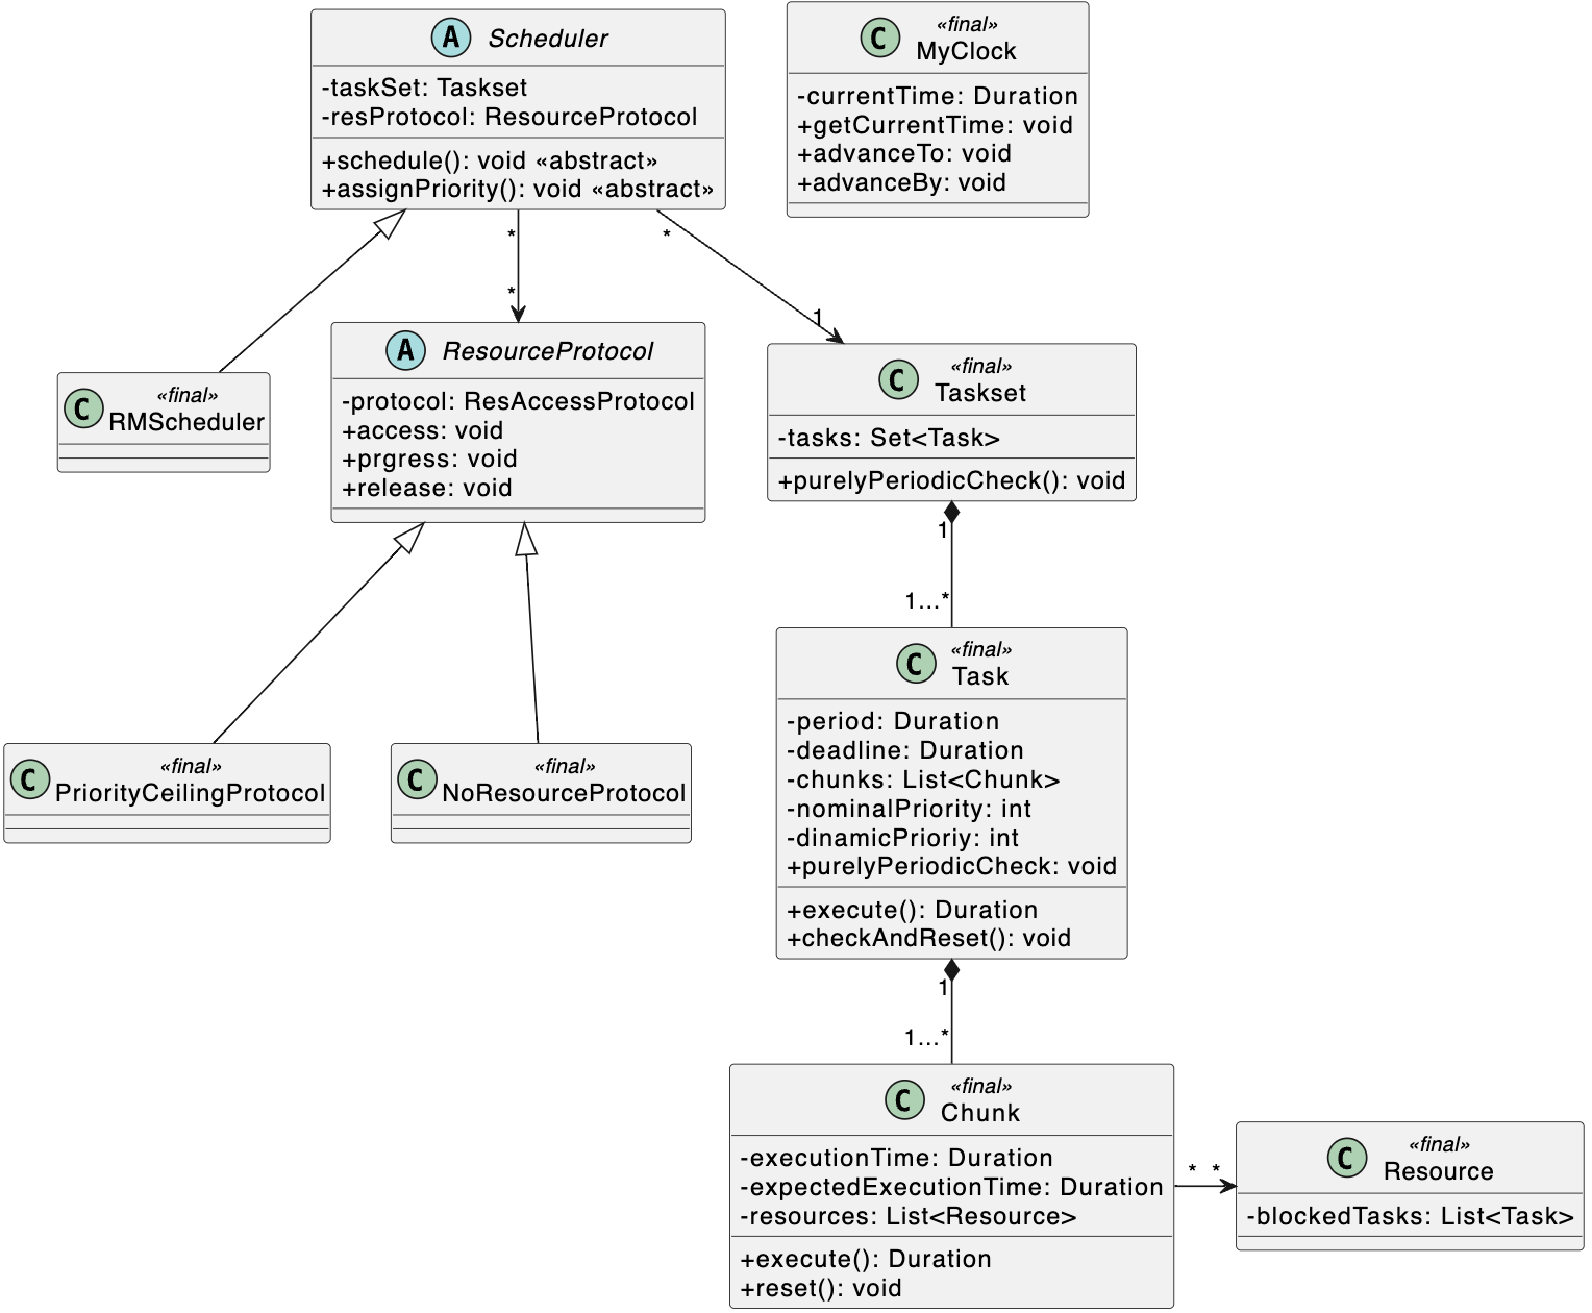
\includegraphics[width=1\textwidth]{immagini/class diagram.pdf}
    \caption{Class diagram.}
\end{figure}